%%%%%%%%%%%%%%%%%%%%%%%%%%%%%%%%%%%%%%%%%%%%%%%%%%%%%%%%%%%%%%%%%%%%%%%%
%    INSTITUTE OF PHYSICS PUBLISHING                                   %
%                                                                      %
%   `Preparing an article for publication in an Institute of Physics   %
%    Publishing journal using LaTeX'                                   %
%                                                                      %
%    LaTeX source code `ioplau2e.tex' used to generate `author         %
%    guidelines', the documentation explaining and demonstrating use   %
%    of the Institute of Physics Publishing LaTeX preprint files       %
%    `iopart.cls, iopart12.clo and iopart10.clo'.                      %
%                                                                      %
%    `ioplau2e.tex' itself uses LaTeX with `iopart.cls'                %
%                                                                      %
%%%%%%%%%%%%%%%%%%%%%%%%%%%%%%%%%%
%
%
% First we have a character check
%
% ! exclamation mark    " double quote  
% # hash                ` opening quote (grave)
% & ampersand           ' closing quote (acute)
% $ dollar              % percent       
% ( open parenthesis    ) close paren.  
% - hyphen              = equals sign
% | vertical bar        ~ tilde         
% @ at sign             _ underscore
% { open curly brace    } close curly   
% [ open square         ] close square bracket
% + plus sign           ; semi-colon    
% * asterisk            : colon
% < open angle bracket  > close angle   
% , comma               . full stop
% ? question mark       / forward slash 
% \ backslash           ^ circumflex
%
% ABCDEFGHIJKLMNOPQRSTUVWXYZ 
% abcdefghijklmnopqrstuvwxyz 
% 1234567890
%
%%%%%%%%%%%%%%%%%%%%%%%%%%%%%%%%%%%%%%%%%%%%%%%%%%%%%%%%%%%%%%%%%%%
%

%AIP Reprint Class%%%%%%%%%%%%%%%%%%%%%%%%%%%%%%%%%%%%%%%%%%%%%%%%%%%%%%%%%%%%%%%%%%%%%%%%%%%%%
%\documentclass[aip,pop,amsmath,amssymb,reprint,superscriptaddress]{revtex4-1} %preprint version
%\usepackage{graphicx}% Include figure files
%\usepackage{dcolumn}% Align table columns on decimal point
%\usepackage{bm}% bold math
%\usepackage{epstopdf}
%
%    \renewcommand{\topfraction}{0.9}    % max fraction of floats at top
%    \renewcommand{\bottomfraction}{0.8}    % max fraction of floats at bottom
%    \setcounter{topnumber}{2}
%    \setcounter{bottomnumber}{2}
%    \setcounter{totalnumber}{4}     % 2 may work better
%    \setcounter{dbltopnumber}{2}    % for 2-column pages
%    \renewcommand{\dbltopfraction}{0.9}    % fit big float above 2-col. text
%    \renewcommand{\textfraction}{0.07}    % allow minimal text w. figs
%    \renewcommand{\floatpagefraction}{0.7}    % require fuller float pages
%    \renewcommand{\dblfloatpagefraction}{0.7}    % require fuller float pages
%    \setlength{\abovecaptionskip}{5pt}
%    \setlength{\belowcaptionskip}{5pt}
%    \setlength{\parskip}{0pt}
%    \setlength{\textfloatsep}{5pt} 

%%%%%%%%%%%%%%%%%%%%%%%%%%%%%%%%%%%%%%%%%%%%%%%%%%%%%%%%%%%%%%%%%%%%%%%%%%%%%%%%%%%%%%%%%%%%%%%%%%

%IOP preprint class %%%%%%%%%%%%%%%%%%%%%%%%%%%%%%%%%%%%%%%%%%%%%%%%%%%%%%%%%%%%%%%%%%%%%%%%%%%%%%
\documentclass[12pt]{iopart}
\newcommand{\gguide}{{\it Preparing graphics for IOP journals}}
%Uncomment next line if AMS fonts required
\usepackage{iopams}
\usepackage{graphicx}
\usepackage{epstopdf}  
%%%%%%%%%%%%%%%%%%%%%%%%%%%%%%%%%%%%%%%%%%%%%%%%%%%%%%%%%%%%%%%%%%%%%%%%%%%%%%%%%%%%%%%%%%%%%%%%%%





\begin{document}

\title{Turbulence analysis of an experimental flux rope plasma}

\author{D.A. Schaffner$^{1}$, V.S. Lukin$^{2}$, A. Wan$^{1}$ and M.R. Brown$^{1}$}

\address{$^{1}$ Swarthmore College, Swarthmore, PA, USA}
\address{$^{2}$ Naval Research Laboratory, Washington, DC, USA}
%\ead{dschaff2@swarthmore.edu} %uncomment for AIP reprint version
\begin{abstract}
We have previously generated elongated Taylor double-helix flux rope plasmas in the SSX MHD wind tunnel.  These plasmas are remarkable in their rapid relaxation (about one Alfv\'en time) and their description by simple analytical Taylor force-free theory despite their high plasma $\beta$ and high internal flow speeds. We report on the turbulent features observed on these plasmas including frequency spectra, autocorrelation function, and probability distribution functions of increments.  We discuss here the possibility that the turbulence facilitating access to the final state supports coherent structures and intermittency revealed by non-Gaussian signatures in the statistics.  Comparisons to a Hall-MHD simulation show a similarity in several statistical measures.
\end{abstract}

%Uncomment for PACS numbers title message
%\pacs{00.00, 20.00, 42.10}
% Keywords required only for MST, PB, PMB, PM, JOA, JOB? 
%\vspace{2pc}
%\noindent{\it Keywords}: Article preparation, IOP journals
% Uncomment for Submitted to journal title message


%\submitto{\PPCF}%uncomment for AIP reprint version
% Comment out if separate title page not required
\maketitle

\section{Overview}

Flux ropes observed in the heliosphere have two striking properties.   First is their rapid emergence.  Whether in the magnetosphere or in the solar corona, these large scale structures emerge rapidly, often in just a few Alfv\'en crossing times of the system.  Second is their long lifetimes.  Once formed, these structures persist for long times despite being embedded in turbulent MHD plasma.  

Flux ropes have recently been observed {\it in situ} at the subsolar magnetopause \cite{Oieroset11}.  In this remarkable coordinated observation using three THEMIS spacecraft, a flux rope is caught in the process of forming, revealing properties that are fundamentally 3D. Since magnetospheric flux ropes evolve rapidly, observations of flux ropes in the magnetosphere tend to be detected at later stages of their evolution.  The newly formed flux rope reported here appeared to be flanked by two active X-lines as part of the formation process.

Flux ropes are also observed remotely in the solar atmosphere \cite{Patsourakos13}.  On July 19, 2012, an eruption occurred on the solar surface producing dynamical magnetic activity resulting in a destabilized flux rope, the acceleration of a fast ($1000~km/s$) coronal mass ejection, and a long-lived solar flux loop.  The long-lived structure is remarkable in its nearly semi-circular topology, and the persistence of a ``coronal rain'' from the loop top for nearly 24 hours.  The observation was made with the Solar Dynamics Observatory's AIA instrument on the sun's lower right hand limb.   This represents the first direct evidence of a fast CME driven by the prior formation and destabilization of a coronal magnetic flux rope.

It is interesting to note that in MHD simulations, the peak in the mean square current density $\langle j^2 \rangle$ is also achieved rapidly, within a fraction of an Alfv\'en time. At this time, the turbulence is fully developed, the peak of small scale activity is achieved, and coherent structures appear. 

We have recently reported on the observation of a long-lived helical flux rope called a Taylor double-helix in the SSX MHD wind tunnel \cite{Gray13}.  The Taylor double-helix is the natural relaxed state of MHD plasma confined in a long, perfectly conducting cylinder \cite{Taylor86}.  In the case of an infinite cylinder, the minimum energy state has a helical pitch of $ ka = 1.234$, where k is the wave number associated with the z axis.  

In the SSX experiments, a magnetized plasma gun launches a magnetized plasma plume into a long flux conserving cylinder.  The plasma rapidly relaxes to the double-helix state in about 1 Alfv\'en crossing time and subsequently decays resistively.  In the paper, we postulated that the physics of selective decay was at play as the initially turbulent plasma relaxed to the double-helix state.  The selective decay hypothesis posits that the energy selectively decays relative to the magnetic helicity because the energy spectra peaks at higher wave numbers, where dissipation is higher \cite{Matthaeus80}.  The wind tunnel's minimum energy state possesses $ka = 1.292$, which is within 5\% of the infinite cylinder's $ka = 1.234$. 

Servidio et al. \cite{Servidio08,Servidio11} detail simulations which observe the rapid and simultaneous magnetohydrodynamic relaxation into localized patches of plasma with near alignment of {\bf J} and {\bf B}. These patches of locally relaxed plasma can then negotiate with adjacent patches to reach a globally relaxed state on a longer time scale.  However, many of the characteristics of the relaxed state will be evident locally. This localized relaxation might explain the rapidity of the transition observed in the double-helix plasmas.  A fully relaxed Taylor state would be expected to have a flat lambda profile (where $\nabla \times B = \lambda B$ governs the equilibrium).  The reported lack of a flat radial lambda profile could also be a consequence of a patchy relaxation.

We suspect that the MHD turbulent flow in the SSX wind tunnel contains patches of locally relaxed plasma with reconnection sites at the boundaries.  A fully relaxed flow might be expected to exhibit Gaussian statistics in its fluctuations and power law behavior for the power spectra; conversely, a flow containing coherent structures and reconnection sites should exhibit non-Gaussian statistics.  Simulations show that coherent structures appear rapidly, in less than one dynamical time.  Large numbers of reconnection sites can be identified statistically in MHD turbulence studies \cite{Servidio09,Servidio10a}.  A statistical way to find these coherent structures is to identify rapid changes in the magnetic field vector.  A useful technique is to generate a probability distribution function (PDF) of vector increments \cite{Greco08,Greco09}.

Greco, {\it et al} \cite{Greco08} identified intermittent structures in MHD turbulence simulations using statistical techniques, then connected the structures with regions of high current density.  Using data from a high resolution 3D MHD simulation, they constructed PDFs of magnetic field vector increments $\Delta {\bf B} = |{\bf B}(s + \Delta s) - {\bf B}(s)|$ for two scale separations $\Delta s$; one much smaller than the correlation scale and another about 2 $\lambda_C$.  They found that the PDF of $\Delta {\bf B}$ at the larger increment was close to Gaussian indicating that increments larger than the correlation scale are normally distributed.  However, the PDF at the smaller increment had substantial tails in the distribution and furthermore, had the same distribution as the PDF of a component of the current density, indicating that the non-Gaussian statistics were correlated with intense current sheets.  They also compared the identification of  discontinuities using the spatial interval method described above with coherent structures identified using (PVI) intermittency statistics and found the techniques to be similar.

In a follow-up investigation, Greco, {\it et al} \cite{Greco09} studied the statistics of ACE solar wind data as well as 2D and 3D simulation data using the same techniques.  Time series were analyzed for the solar wind data while spatial separations were analyzed from the simulations.  First, they found that the ACE solar wind data had nearly identical increment PDFs to the 2D simulation data.  Second, they were able to correlate specific features in the 2D simulation to departures from Gaussian statistics in the PDF.  A narrow inner peak is super-Gaussian and corresponds to small fluctuations in the lanes between magnetic islands.  An intermediate range is sub-Gaussian and corresponds to fluctuations in current cores inside magnetic flux tubes.  Finally, at several standard deviations, there are super-Gaussian wings corresponding to coherent small-scale current-sheet-like structures that form the sharp boundaries between the magnetic flux tubes.

Non-Gaussian statistics and characteristic coherent structures are initiated almost identically in dissipative and ideal systems \cite{Wan09}. Therefore we postulate that the origins of coherence and intermittency are essentially ideal, with dissipation acting only to limit growth of the smallest scale structures.  The fact that our Lundquist number is modest (S = 1000) should not impact the emergence of coherent structures.

We are interested here in the post-selective decay phase of the double-helix, in particular, processes that rapidly evolve the state such as patchiness and the evolution of coherent structures. First we report on the turbulent temporal power spectrum for various aspects of these experimental flux ropes and fit to power-laws in order to compare to similar measurements in both the solar wind and MHD simulations. Then, we present MHD turbulence statistics that suggest the emergence of non-Gaussian structures. These experimental turbulent features are compared to simulation data generated by the HiFi code using both a resistive-MHD and Hall-MHD framework designed to have a geometry and plasma parameters matched to the experiment.

\section{Experiment}

The flux ropes under investigation are formed in a wind-tunnel configuration of the Swarthmore Spheromak Experiment. A copper cylindrical flux conserver serves as the tunnel capped by two plasma gun electrodes whose extent limits the length of the tunnel to $86~cm$ as can be seen in Figure~\ref{fig:SSXdiagram}. The radius, R,  of the cylinder is $7.75~cm$ making the aspect ratio of the this configuration, L/R = 11. Though slightly shorter than the tunnel reported in previous work~\cite{Gray13}, the aspect ratio is considered still large enough for comparison to an infinite cylinder in Taylor relaxation theory. The plasma itself is formed by the discharge of a $1~mF$, $3.5~kV$ capacitor across a few centimeters wide gap between the tungsten-coated gun inner electrode and outer wall into a puffed volume of hydrogen gas. After ionization, currents of over $80~kA$ across the gap push plasma into the main section of the flux conserver through $j \times B$ forces. Magnetic coils coaxial to the gun electrode and flux conserver contributes the stuffing flux which allows for the formation of a spheromak at the gun edge. Given the high aspect ratio, the spheromak tilts, eventually forming a twisted double-helix Taylor state; this sequence has been shown to occur in a very short time span~\cite{Gray13}. For this discharge configuration, the amount of current needed to push spheromaks off of the gun and into the main chamber is maintained for approximately $30~\mu s$ ($\sim 20-50~\mu s$ from initial discharge). The discharge likely begins with the formation of a spheromak structure into the chamber vacuum, which may or may not completely break-off from the gun source before more plasma is introduced behind it. Thus these shots generally consist of a sustained injection of structured plasma rather than a single well-defined spheromak---a configuration called slow formation~\cite{jarboe83} . As this paper will discuss, the turbulence nature of this plasma unaffected by the source physics as the selective decay of the plasma likely occurs locally.

Magnetic fluctuations are measured using an arrayed $\dot{B}$ probe; $\dot{B}$ in three directions (r, $\theta$ and z) is measured using 3 orthogonally-oriented $0.3~cm$ single-loop coils at 16 locations separated by $0.4~cm$ beginning $1~cm$ from the cylindrical axis. Signals are acquired using a DTaq digitizer at 14-bit resolution and 65MHz sampling rate. Magnetic field vectors are computed through numerical integration of the $\dot{B}$ signal. Mach number fluctuations, as a proxy for velocity fluctuations, are measured using a Mach probe oriented along the axial/z-axis~\cite{Zhang11} and located $1.5~cm$ from the inner edge of the flux conserver. Density measurements are made using a He-Ne (633nm) laser interferometer through a diameter of the flux conserver set a distance axially of $21.5~cm$ from the midplane (closer to the plasma source). In the data presented here, it is assumed that the plasma has already achieved a relaxed Taylor state by the time it reaches the midplane where most of the diagnostics are located. The chamber is pumped down to $\sim 6 \times 10^{-8}~Torr$ and undergoes a helium glow discharge between runs so it is assumed that any influence on the plasma by impurities is low.

An additional important point regarding this experiment is that due to nature of the plasma production method, the plasma does not have a typical guide field direction; that is, the turbulence tends to be isotropic. This is evident in the similarity of the spectra for the three different probe directions.

\begin{figure}[!htbp]
\centerline{
\includegraphics[width=8.5cm]{SSXdiagram.eps}}
\caption{\label{fig:SSXdiagram} (a) SSX Diagram with the two plasma gun configuration. The plasma is confined to the cylindrical flux conserver in the manner of the simulated images in b and c. Magnetic and Mach probes are indicated at the midplane while interferometer density is measured $21.5~cm$ off the midplane. (b)HiFi Simulation: B-field structure at an early time, before selective decay. The plasma source is the on the left. (c) B-field structure at a later time after selective decay.}
\end{figure}

\section{HiFi Simulation}

\section{Results}

The SSX produces flux-rope plasma that persists on the order of $120~\mu s$. Figure~\ref{fig:timeseries36} shows a timeseries of numerically integrated B-field---$|B|=\sqrt{B_{r}^{2}+B_{\theta}^{2}+B_{z}^{2}}$---for the innermost tip ($1~cm$ from the cylindrical axis), interferometer line-averaged density, $n$, Mach probe measurement of Mach number, M, and discharge current, $I_{gun}$, for a sample shot and for an average of 35 shots. For time analysis, the shots are divided into epochs to account for the dynamical nature of the plasma discharges as indicated by the dashed lines in Figure~\ref{fig:timeseries36}. The formation/selective-decay epoch spans from 30 to 40 $\mu s$. As shown in a previous publication~\cite{Gray13}, the selective-decay of the plasma into a Taylor state likely occurs in this time range. The equilibrium epoch ranges from 40 to 60 $\mu s$ and is the period of turbulent fluctuations most closely analyzed here. This time range sees a generally stable period of fully developed turbulence balanced between the sourced plasma from the gun and resistive/viscous effects that degrade the magnetic fields and flows. The epoch from 60 $\mu s$ on is considered the decay epoch and represents the flux-rope structure's resistive and viscous dissipation. Clearly, as in Figure~\ref{fig:timeseries36}(a), the magnetic field resistively decays away by $120 \mu s$. Remaining unmagnetized plasma, however, has been shown to persist for many hundreds of microseconds.

\begin{table}
\caption{\label{tab:params}Plasma parameters during the equilibrium epoch for this configuration of SSX.}
\begin{tabular}{ll}
Parameter&Value\\
\hline
$V_{a}$&$240km/s$\\
$f_{ci}$&$7.6MHz$\\
Axial $\tau_{A}$&3.5$\mu$s\\
Radial $\tau_{A}$&0.3$\mu$s\\
$\rho_{i}$&0.091cm\\
$\delta_{i}$&0.51cm\\
$C_{s}$&31km/s\\
$\beta$&0.0967\\
\end{tabular}
\end{table}

In the equilibrium epoch, the average magnetic field is $5~kG$ and average density is $2\times 10^{15}~cm^{-3}$; thus, radial and axial Alfv\'en transit times are 0.3 and $3.5\mu s$ respectively. Ion temperature is measured using an ion Doppler spectrometer system at the midplane. Background ion temperatures (i.e. average temperatures made avoiding large heating events) are on the order of $20~eV$. Though not measured in this dataset, previous measurements of electron temperature suggest a value of $10~eV$ for this system. Combined with the average field and density values measured, estimates of ion gyrofrequency ($f_{ci}$), ion gyroradius ($\rho_{i}$) and ion inertial length ($\delta_{i}$) can be made. These values are listed in Table~\ref{tab:params}. Of particular note, the ratio of system size to $\rho_{i}$ is large, R/$\rho_{i} \cong 80$, suggesting that the influence of the wall on plasma dynamics is minimal.

The density trace in Figure~\ref{fig:timeseries36}(b) shows peaking in the formation epoch, but an eventual drop to approximately $1\times 10^{15}$cm$^{-3}$ for the majority of the discharge. The initial peaking is likely due to the initial spheromak formation, where plasma is being pushed into the tunnel, but before the threshold for break-off is achieved. The Mach number trace is on average positive, indicating flow predominately away from the gun source as would be expected. The average Mach number during the equilibrium epoch is M=0.4 which for the sound speed listed in Table~\ref{tab:params} yields an average flow speed of 12km/s. It is likely that flow speeds toward the center can be even higher. Indeed, a time of flight estimate based on the axial separation distance between the interferometer measurement and the midplane $\dot{B}$ measurement suggests a bulk plasma flow of 20km/s. As seen in the single shot trace in Figure~\ref{fig:timeseries36}, there can sometimes be flow reversal which most likely indicates a reflection of flow off of the far axial boundary.

It can also be observed that the decay time for magnetic field and Mach number, during the dissipation epoch, are on the same order. This suggests a Prandtl number of order one. That is, resistive and viscous effects are on the same order for these discharges.

\begin{figure}[!htbp]
\centerline{
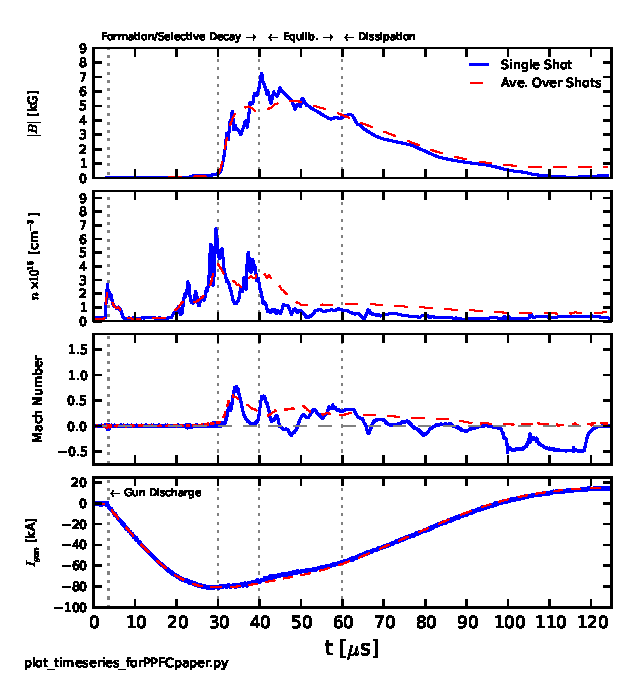
\includegraphics[width=8.5cm]{timeseries36.eps}}
\caption{\label{fig:timeseries36} Timeseries of (a) Magnetic Field magnitude, (b) Density, (c) Mach Number, and (d) Discharge current. An example single shot is shown (blue line) as well as the average trace for 35 shots (red line).}
\end{figure}

\subsection{Spectra}

Given the dynamical nature of these plasmas, the spectral decomposition has been achieved using a Wavelet technique rather than with Fast Fourier Transforms (FFTs). This wavelet technique has been shown to be useful in situations where data may be non-stationary and provides a more accurate method for simultaneous spectral and temporal decomposition than a windowed Fourier transform because it applies a transform at many scales rather than a single scale~\cite{torrence98}. To achieve better resolution in frequency space, a sixth-order Morlet mother wavelet has been used. Morlet wavelet scales (i.e. frequencies) are generally well matched to Fourier scales, though since we are most interested here in power spectral densities (PSD), the choice of wavelet is not critical~\cite{torrence98}. A wavelet decomposition for a single shot $\dot{B}$ timeseries is shown in Figure~\ref{fig:waveletcontour} with the wavelet scale converted to a Fourier frequency as the y-axis and time as the x-axis. The color scale corresponds to the normalized fluctuation power. Changes in the spectral nature can be seen with time: higher frequency fluctuations grow up and peak around 30$\mu s$, hold stable until about 60$\mu s$, and then begin to dissipate. This change in fluctuations supports the division of the data into epochs.

\begin{figure}[!htbp]
\centerline{
\includegraphics[width=8.5cm]{waveletcontour.eps}}
\caption{\label{fig:waveletcontour} Wavelet Power Spectrum of $\dot{B}_{\theta}$ as a function of time for a single shot (same as that shown in Figure~\ref{fig:timeseries36})}
\end{figure}

The reduced power spectra for B-field, density and Mach number fluctuations are displayed in Figure~\ref{fig:waveletspec}. The B-field curves are produced by first taking a wavelet transform of the $\dot{B}$ timeseries (for any one of the orthogonal components), yielding an array with $\dot{B}$ fluctuation power as a function of both time and frequency as in Figure~\ref{fig:waveletcontour}, and scaling the $\dot{B}$ power by $f^{2}$ in order to recover actual B-field fluctuation power. This approach is derived from the assumption that the B-field fluctuations are able to be Fourier decomposed such that
%
\begin{equation}
\frac{d}{dt}B(t) = \frac{d}{dt}B_{0}e^{i2\pi f} \sim ifB
\end{equation}
%
resulting in the relationship between $\tilde{B}(f)$ and $\tilde{\dot{B}}(f)$ as
%
\begin{equation}
|\tilde{B}(f)|^{2} = \frac{1}{f^{2}}|\tilde{\dot{B}}(f)|^{2}
\end{equation}
%
where $|\tilde{x}(f)|^{2}$ is the PSD. The same relationship applies for the Wavelet Transform. Once converted into a B-field power array, the 1-D spectrum is calculated by summing over a certain time region---in this case the equilibrium epoch of 40 to 60$\mu s$. The shot-averaged spectra for the magnetic field components ($B_{r}$, $B_{\theta}$, and $B_{z}$) are nearly identical suggesting that magnetic fluctuations are isotropic. For clarity, only the $B_{\theta}$ component is shown in Figure~\ref{fig:waveletspec}.  A similar approach is made for density and Mach number, though without the frequency scaling.

\begin{figure}[!htbp]
\centerline{
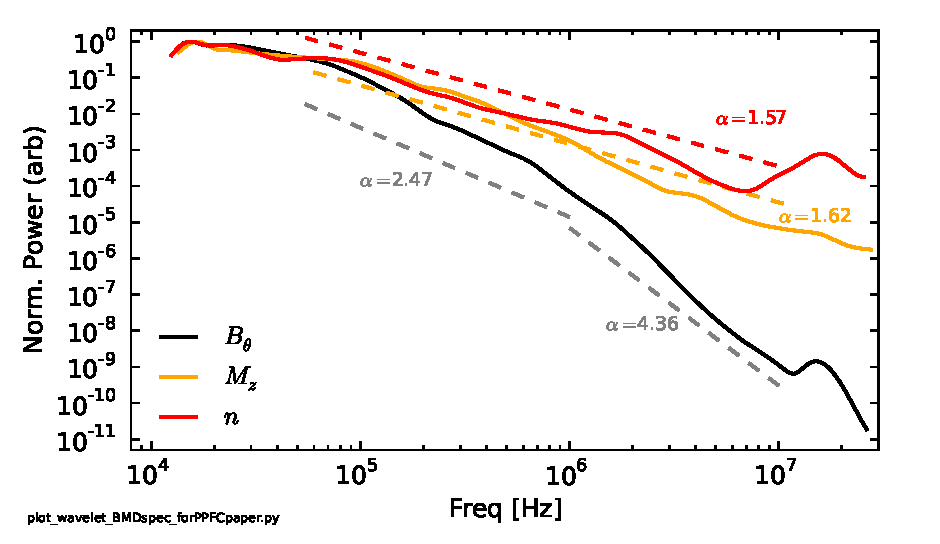
\includegraphics[width=8.5cm]{waveletspec.eps}}
\caption{\label{fig:waveletspec} Wavelet Spectrum of B-field, density, and Mach number fluctuations for the equilibrium epoch, 40 to 60$\mu$s.}
\end{figure}

All three curves shown have roughly linear behavior in the spectral region between 50kHz and 10MHz. A power-law fit of spectral power to frequency ($P(f) \sim f^{-\alpha}$) is made for density and Mach number in this frequency range using a maximum likelihood estimation method~\cite{clauset09} (MLE) yielding exponents of $\alpha = 1.57$ for the density spectrum and $\alpha = 1.62$ for the Mach spectrum, which servers as a proxy for the velocity spectrum in this experiment. An exponent of 1.62 for velocity is very close to the typical Kolmogorov exponent of -5/3 = 1.66 for hydrodynamic flow fluctuations.

The magnetic field spectrum appears to have two separate regions: a shallower sloped region between 50kHz and 1MHz and a steeper sloped region between 1MHz and 10MHz. MLE fits for these regions give exponents of $\alpha = 2.47$ (shallower) and $\alpha = 4.36$ (steeper). Both the plots and the fits indicate that the spectra index for B-field fluctuations is steeper than that for Mach/velocity fluctuations and thus steeper than that measured in the solar wind. This is perhaps indicative of a magnetic field dissipation mechanism that is present in the experimental plasma, but not in space.

The origin of the break in the spectra can potentially come about in a number of ways. First, it may simply be due to the effect of flowing plasma across the probe. The Taylor hypothesis---frozen-in flow---suggests that measured temporal spectra can be mapped to spatial spectra when the medium containing the fluctuations is moving past a probe at some velocity. Thus, in the spectrum, there is some critical frequency below which fluctuations can be considered predominately due to spatial structure, and above which fluctuations are due to some combination of spatial and temporal structure. A rough estimate for this critical frequency can be made by considering the average flow and probe size. The average axial flow for the equilibrium epoch as indicated by the Mach probe and the assumed $C_{s}$ is $12~km/s$; with a $3~mm$ probe size, the critical frequency would be $4~MHz$. Thus the break in slope could be showing a transition between the power spectrum representing the energy transfer in both spatial and temporal scales (higher frequencies) and a spectrum due to the energy transfer in only spatial scales (lower frequencies), since lower frequency temporal fluctuations become less observable by the probe. 

The break could also be related to the temporal decorrelation of the signal. Figure~\ref{fig:autocorr} shows the autocorrelation function for $\dot{B}$ for each of the three axes, again during the equilibrium epoch. A decorrelation time can be defined as the $\tau$ at which the autocorrelation function crosses zero. For $\dot{B}_{r}$ and $\dot{B}_{\theta}$, $\tau = 1.0~\mu s$ which corresponds to a frequency of $1~MHz$---also called a decorrelation rate. If there are any wave modes in the plasma, they could influence the spectrum at frequencies below the decorrelation rate. Indeed, there has been some evidence that mode types can have an effect on energy transfer rates that manifest in the power spectrum~\cite{shaikh09}. Above the decorrelation rate, the fluctuations arise purely from the turbulence which may have a different energy transfer rate. Consequently, this may appear as a change in the spectral index around the decorrelation frequency.

Finally, this break may be due, of course, to a transition to the dissipation range of the spectrum. Possible dissipation scales include the ion gyroradius and ion inertial length which are $\sim 0.1~cm$ and $\sim 0.5~cm$ respectively for the equilibrium epoch. Dissipation could also occur directly in frequency space with coupling to the ion gyrofrequency, which here is $7.6~MHz$. If the Taylor hypothesis is made, and frequencies mapped to wavelengths using the average velocity, the break point occurs at a length of $1.2~cm$; the ion inertial length scale maps to a frequency of $2.4~MHz$.

\begin{figure}[!htbp]
\centerline{
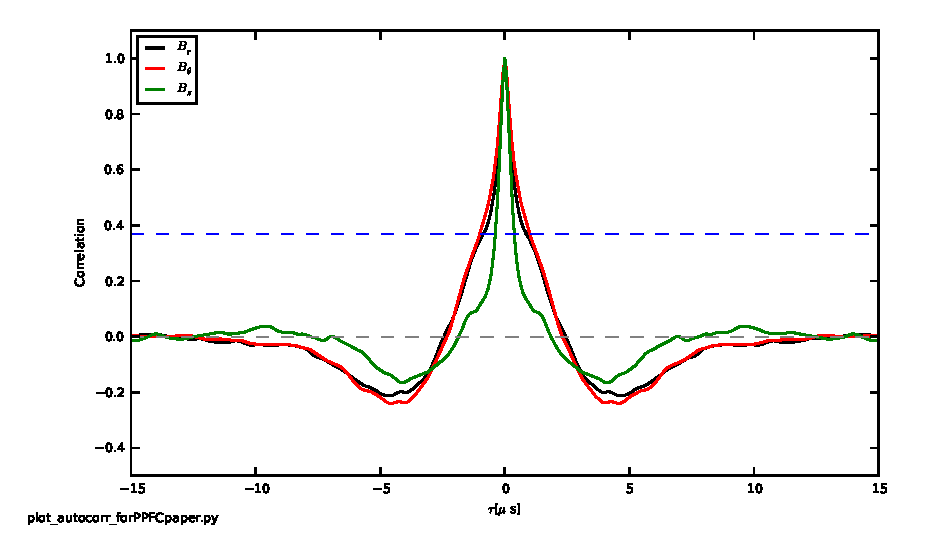
\includegraphics[width=8.5cm]{autocorr.eps}}
\caption{\label{fig:autocorr} Autocorrelation function for $\dot{B}$ fluctuations in the time range 40 to 60 $\mu$s.}
\end{figure}

The HiFi simulation also produces a time series B-field, density and flow. Unlike the experimental data however, the simulated discharge consists of a single spheromak formation and decay with a lifetime on the order of $50 \mu s$. The simulation does not model slow formation, or the sustainment of plasma injection seen in the experiment. However, a comparison between the two can be made by observing the similarity of the simulated pulse with the tail end of the experimental discharge. This can be clearly seen in Figure~\ref{fig:simtimeseries64} where the simulated time series has been shifted to approximately match the decay features of the B-field, as well as a few fluctuation features of the density and Mach number. The experimental shot here was chosen for its particularly well-matched features.

\begin{figure}[!htbp]
\centerline{
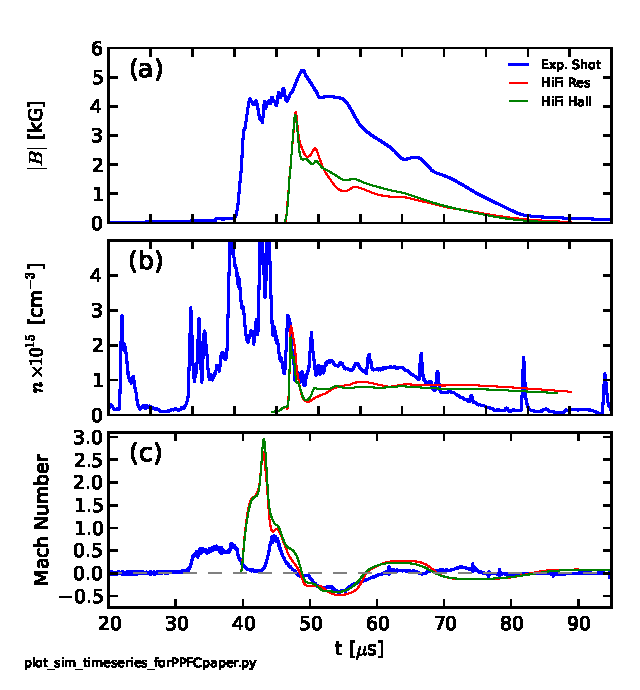
\includegraphics[width=8.5cm]{simtimeseries64.eps}}
\caption{\label{fig:simtimeseries64} Time series of magnetic field, density and Mach number for a Resistive MHD simulation, MHD-Hall simulation and a single experimental shot.}
\end{figure}
\begin{figure}[!htbp]
\centerline{
\includegraphics[width=8.5cm]{simBspectra.eps}}
\caption{\label{fig:simBspectra} Comparison of B-field spectra from Resistive MHD simulation and a Hall-MHD simulation to the experimental spectra. The spectra are computed over a time period from 46 to 66$\mu$s to approximate the equilibrium epoch of the much shorter simulated pulses.}
\end{figure}

This similarity highlights the assertion that despite the longer injection time of plasma in the experiment (and thus, less well-defined large scale structure), the selective decay/self-organization still occurs. Moreover, the similarity allows us to compare the turbulent features of the experiment and the MHD simulation.

Figure~\ref{fig:simBspectra} shows wavelet spectra for the simulation runs as well as the averaged experimental spectra. Due to the short smaller number of points in the timeseries for the simulation, the wavelet decomposition used a fourth-order Paul mother wavelet  which has a slightly better time resolution than the sixth-order Morlet wavelet used above. The experimental data is also reanalyzed using a Paul wavelet for direct comparison to the simulation data, but the differences between the two wavelet transforms is minimal for the experimental data which is sampled at a higher frequency. Like the experimental spectra, there appear to be two linear regions. The slopes of both the resistive-MHD and Hall-MHD simulation spectra are very close to that of the experimental data in the region between 20kHz and 300kHz. The simulation spectra, however, begin to steepen at a lower frequency than the experimental data: $\sim 300kHz$ compared to $\sim 1~MHz$. This is consistent with the autocorrelation function for the simulation which gives decorrelation times on the order of $3.3 \mu s$. The simulation does not appear to shed any light on the possible role of dissipation. The spectra for both resistive and Hall MHD are similar so that any modification of the physics due to the inclusion of a Hall term is not apparent in the data. Nevertheless, the slope of the simulation spectra are very close to the experiment.
%Speculation about ion inertial length with Hall term simulation? 

\subsection{PDFs}

While spectra can be useful for obtaining the relative rate of energy transfer amongst injection, inertial and dissipation scales, they can obscure other signatures of turbulence that can only be seen when looking at higher integral moments. One technique for investigating these higher moments is to construct probability distribution functions (PDF's) from the data at different timescales and then directly calculate moments. The variation in the moments of PDFs as a function of timescale has been shown to be linear for fully-developed fluid turbulence~\cite{frisch95}. One can introduce a timescale into the timeseries by filtering~\cite{frisch95,wan12_apj} or by taking differences of the data points at different time steps~\cite{Greco08,Greco09}. This latter technique is used here where a series of $\Delta \dot{B}$ increments is constructed for a variety of timesteps, $\tau$, as in
\begin{equation}
\Delta \dot{B}_{\tau}(t) = \dot{B}(t+\tau)-\dot{B}(t)
\label{eq:increments}
\end{equation}

\begin{figure}[!htbp]
\centerline{
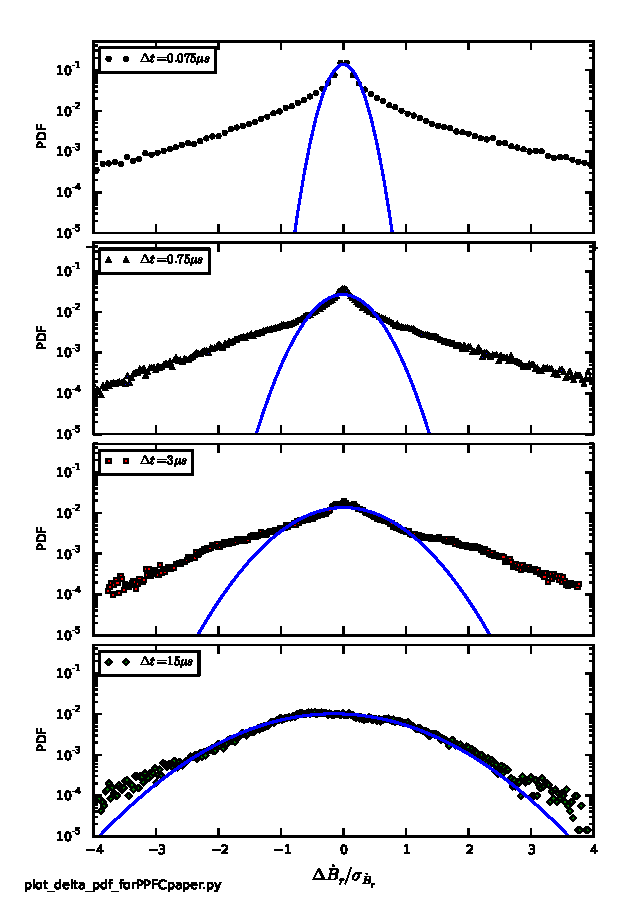
\includegraphics[width=8.5cm]{pdfs.eps}}
\caption{\label{fig:pdfs} PDFs of $\Delta \dot{B}$ in the time range 40 to 60 $\mu$s normalized to the standard deviation for each list.}
\end{figure}
\begin{figure}[!htbp]
\centerline{
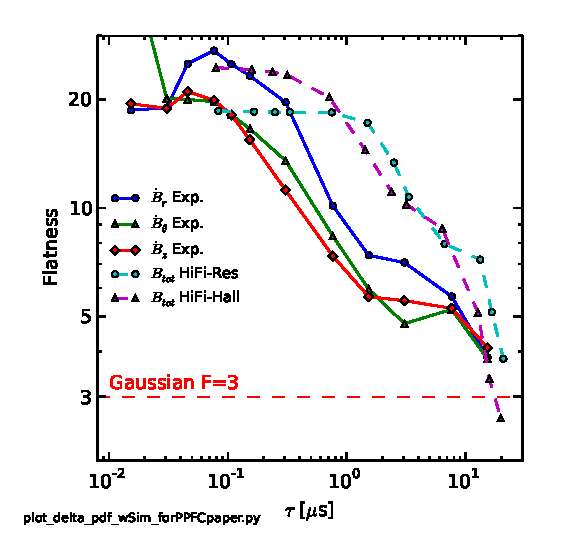
\includegraphics[width=8.5cm]{flatness.eps}}
\caption{\label{fig:flatness} The flatness of the PDFs as a function of $\tau$ on a log-log scale. A flatness of 3 would indicate a perfectly Gaussian distribution. A linear slope between 0.1 and 1$\mu$s---corresponding to the frequency range of 1MHz to 10MHz---suggest a power-law like relationship between the flatness and the timestep. The flatness curves for the HiFi simulations are also listed. They show a similar shape, but seem to be offset in $\tau$.}
\end{figure}

A series of these PDFs for the equilibrium epoch timeseries is shown in Figure~\ref{fig:pdfs} for $\tau$'s of $0.15~\mu s$, $0.75~\mu s$, $3~\mu s$ and $15~\mu s$ which corresponds to filtering the timeseries above frequencies of $6.6~MHz$, $1.3~MHz$, $333~kHz$, and $66~kHz$ respectively. The PDFs are normalized to the root mean square value of the increments and to the total area. A Gaussian function is fit to each distribution. One can clearly see a transition from non-Gaussian distributions for small $\tau$'s to more Gaussian distribution for larger $\tau$'s. The features of the non-Gaussian distributions are indicative of intermittency in the signal; the fat tails signify large swings in the values of the timeseries and the timestep indicates the relative temporal size of the intermittent events.

The level of intermittency as a function of $\tau$ can be quantified using a calculation of the flatness defined as~\cite{deWit13}
\begin{equation}
F(\tau) = \frac{S_{4}(\tau)}{S_{2}(\tau)^{2}}
\label{eq:flatness}
\end{equation}
where $S_{p}(\tau)$ is the p-th order moment for the distribution of increments, $\Delta \dot{B}$, as in
\begin{equation}
S_{p}(\tau) = \int_{-x_{max}}^{x_{max}} P(\Delta \dot{B})(\Delta \dot{B})^{p} dx
\label{eq:structurefunc}
\end{equation}
with x representing a histogram bin width. An exact Gaussian distribution would have a flatness equal to 3.

The resulting function for flatness is shown in Figure~\ref{fig:flatness} for each of the three $\dot{B}$ measurements. The plot shows the trend toward Gaussian (as represented by the dashed line at F=3) as the timestep is increased. An increase in flatness signifies an increase in the intermittency observed in the PDF---the flatness grows rapidly beyond $\tau$ = 1$\mu s$ corresponding to a frequency of $1~MHz$. Since fluctuations beyond this frequencies are more and more temporally correlated (as indicated by the autocorrelation function), it is clear that the intermittent nature is truly imbedded in the magnetic signal. Conversely, a trend toward Gaussian distribution might be expected for fluctuations that are not temporally correlated; however, recent work in this vein on solar wind measurements has speculated that such a change in flatness versus timescale might be expected at the transition from inertial to dissipation range turbulence~\cite{wan12_apj}. This perhaps indicates that dissipation physics might yet be in play at these scales.

The simulation data can also be analyzed within the PDF of increments framework. The flatness curve is also shown in Figure~\ref{fig:flatness} for the two different simulation runs. The shape of the curve is very similar to the experimental one, though the changes in flatness are offset in time increment as higher values of flatness are reached at larger increments. The largest values of flatness for both experimental and simulation are similar suggesting that the mechanism responsible for the intermittency might be common to both.

\section{Conclusion}

We have hypothesized that the turbulent relaxation of a twisted flux rope plasma in the SSX wind tunnel was promoted by intermittency and coherent structures.  The rapidity of the relaxation process (about one Alf\'ven time) could be due to fast local relaxation of the coherent structures followed by a slower relaxation of the structure as a whole.  In this study, we have focused on time series and temporal frequency statistics: autocorrelation function, power frequency spectra, and PDFs of temporal increments.  Spatial correlations and spectra will be reported in a later article.

Magnetic field power frequency spectra from the experiment show power-law behavior over two decades but with steeper spectral indices than measured in the solar wind and predicted from theory. Comparisons of power frequency spectra with HiFi simulation show good correspondence with indices $\alpha \approx 2.5$ at low frequencies and steeper at higher frequencies.  The reason for the break in the spectra slope has not been identified; however, both experimental and simulation data had measured decorrelation rates which could be placed near the respective break points. Furthermore, it's not clear whether a dissipation scale has been observed in the SSX plasma in these experiments.

Probability distribution functions PDFs of the magnetic field increments expose non-Gaussian higher order statistics connected to intermittency and coherent structures.  We find large values of flatness at short time increments corresponding to small spatial scales in both the experiment and simulation.  In addition, we find that the shape of the curve of flatness with increasing time increment is very similar in both experiment and simulation.

The observation of non-Gaussian values for flatness in the PDFs, and the trend for increasing flatness with decrease in timestep is a strong indication for the presence of intermittent fluctuations and/or coherent structures in the plasma which could not be observed with spectra alone. The physical origin of these coherent structures in the SSX plasma has not yet been identified. As seen in previous simulation work~\cite{Servidio11b}, the coherent structures can be matched to the presence of current sheets which in turn could be the site of a reconnection layer. Given the observation of reconnection in past SSX work~\cite{Cothran09,Gray10}, there is a strong likelihood that such events are present in the current SSX configuration though perhaps at a smaller scale.

\section*{References}
\begin{thebibliography}{10}
\bibitem{Oieroset11}
Oieroset, M., T. D. Phan, J. P. Eastwood, M. Fujimoto, W. Daughton, M. Shay, V. Angelopoulos, F. S. Mozer, J. P. McFadden, D. E. Larson, and K. -H. Glassmeier, Direct evidence for a three-dimensional magnetic flux rope flanked by two active magnetic reconnection X-lines at the Earth's magnetopause, Physical Review Letters, Vol. 107, 165007, 2011

\bibitem{Patsourakos13}
S. Patsourakos, A. Vourlidas, and G. Stenborg. Direct Evidence for a Fast Coronal Mass Ejection Driven by the Prior Formation and Subsequent Destabilization of a Magnetic Flux Rope,
ApJ 764 125, 2013

\bibitem{Gray13} 
T. Gray, M. R. Brown, and D. Dandurand, Observation of a Relaxed Plasma State in a Quasi-Infinite Cylinder, Phys. Rev. Letters 110, 085002 (2013). 

\bibitem{Gray10}
Three-dimensional reconnection and relaxation of merging spheromak plasmas 
T. Gray, M. R. Brown, C. D. Cothran, and V. S. Lukin 
Physics of Plasmas 17, 102106 (2010)

\bibitem{Cothran09}
C. D. Cothran, M. R. Brown, T. Gray, M. J. Schaffer, and
G. Marklin, Phys. Rev. Lett. 103, 215002 (2009).

\bibitem{Taylor86} J. B. Taylor, Rev. Mod. Phys. 58, 741 (1986).

\bibitem{Matthaeus80} W.H. Matthaeus and D. Montgomery, Ann. N.Y. Acad. Sci. 357, 203 (1980).

\bibitem{Servidio08}
Servidio, S., Matthaeus, W. H., and Dmitruk, P.: Depression of Nonlinearity in Decaying Isotropic MHD Turbulence, Phys. Rev. Lett., 100, 095005, doi:10.1103 Phys. Rev. Lett.100.095005, 2008.

\bibitem{Servidio11}
Servidio, S., Dmitruk, P., Greco, A., Wan, M., Donato, S., Cassak, P. A., Shay, M. A., Carbone, V., Matthaeus, W. H., Magnetic reconnection as an element of turbulence, Nonlinear Processes in Geophysics, Vol. 18, p. 675-695, 2011. 

\bibitem{Servidio09}
Servidio, S., Matthaeus, W. H., Shay, M. A., Cassak, P. A., and Dmitruk, P.: Magnetic Reconnection in Two-Dimensional Magnetohydrodynamic Turbulence, Phys. Rev. Lett., 102, 115003, doi:10.1103/PhysRevLett.102.115003, 2009.

\bibitem{Servidio10a}
Servidio, S., Matthaeus, W. H., Shay, M. A., Dmitruk, P., Cassak, P. A., and Wan, M.: Statistics of magnetic reconnection in two- dimensional magnetohydrodynamic turbulence, Phys. Plasmas, 17, 032315, doi:10.1063/1.3368798, 2010a.

\bibitem{Servidio10b}
Servidio, S., Wan, M., Matthaeus, W. H., and Carbone, V.: Local relaxation and maximum entropy in two-dimensional turbulence: Phys. Fluids, 22, 125107, doi:10.1063/1.3526760, 2010b.

\bibitem{Servidio11b}
Servidio, S., Greco, A., Matthaeus, W. H., Osman, K. T., and Dmitruk, P.: Statistical association of discontinuities and reconnection in magnetohydrodynamic turbulence, J. Geophys. Res., 116, A09102, 1Ð11, doi:10.1029/2011JA016569, 2011.

\bibitem{Greco08}
Greco, A., Chuychai, P., Matthaeus, W. H., Servidio, S., and Dmitruk, P.: Intermittent MHD structures and classical discontinuities, Geophys. Res. Lett., 35, L19111, doi:10.1029/2008GL035454, 2008.

\bibitem{Greco09}
Greco, A., Matthaeus, W. H., Servidio, S., Chuychai, P., and Dmitruk, P.: Statistical Analysis of Discontinuities in Solar Wind ACE Data and Comparison with Intermittent MHD Turbulence, Astrophys. J., 691, L111, doi:10.1088/0004-637X/691/2/L111, 2009.

\bibitem{Wan09}
Wan, M., Oughton, S., Servidio, S., and Matthaeus, W. H.: Generation of non-Gaussian statistics and coherent structures in ideal magnetohydrodynamics, Phys. Plasmas, 16, 080703, doi:10.1063/1.3206949, 2009.

\bibitem{Wan12}
Wan, M., W. H. Matthaeus, H. Karimabadi, V. Roytershteyn, M. Shay, P. Wu, W. Daughton, B. Loring, and S. C. Chapman, Intermittent Dissipation at Kinetic Scales in Collisionless Plasma Turbulence, Physical Review Letters, Vol. 109, 195001, 2012. 

\bibitem{Osman11}
Osman, K. T., Matthaeus, W. H., Greco, A., and Servidio, S.: Evidence for Inhomogeneous Heating in the Solar Wind, Astrophys. J., 727, L11, doi:10.1088/2041-8205/727/1/L11, 2011.

\bibitem{Zhang11}
X. Zhang, D. Dandurand, T. Gray, M. R. Brown, and V. S. Lukin, "Calibrated Cylindrical Mach Probe in a Plasma Wind Tunnel", Review of Scientific Instruments 82, 033510 (2011).

\bibitem{torrence98}
C. Torrence, G.P. Compo, A practical guide to wavelet analysis. Bull. Am. Meteorol. Soc. 79, 61–78 (1998). doi:10.1175/1520-0477(1998)079<0061:APGTWA>2.0.CO;2

\bibitem{deWit13}
T. Dudok de Wit, O. Alexandrova, I. Furno, L. Sorriso-Valvo, G. Zimbardo, Methods for Characterising Microphysical Processes in Plasmas. Space Sci. Rev. 0038-6308 (2013). 10.1007/s11214-013-9974-9

\bibitem{clauset09}
A. Clauset, C. Rohilla Shalizi, M.E.J. Newman, Power-law distributions in empirical data. SIAM Rev. 51, 661–703 (2009). doi:10.1137/070710111

\bibitem{frisch95}
Frisch, U. 1995, Turbulence (Cambridge: Cambridge Univ. Press)

\bibitem{wan12_apj}
Investigation of intermittency in magnetohydrodynamics and solar wind turbulence: scale-dependent kurtosis, Minping Wan et al., The Astrophysical Journal 744, 171 (2012)

\bibitem{shaikh09}
3D Simulations of Fluctuation Spectra in the Hall-MHD Plasma, D. Shaikh and P.K. Shukla, Physical Review Letters, 102, 045004 (2009). DOI:	10.1103/PhysRevLett.102.045004

\bibitem{jarboe83}
Slow Formation and Sustainment of Spheromaks by a Coaxial Magnetized Plasma Source, T. R. Jarboe, I. Henins, A. R. Sherwood, Cris W. Barnes, and H. W. Hoida,
Phys. Rev. Lett. 51, 39–42 (1983)


\end{thebibliography}

\end{document}

